\documentclass{article}
\usepackage[preprint]{neurips_2024}
\usepackage[utf8]{inputenc}
\usepackage[T1]{fontenc}
\usepackage[hidelinks]{hyperref}
\usepackage{url}
\usepackage{booktabs}
\usepackage{amsfonts}
\usepackage{amsmath}
\usepackage{amssymb}
\usepackage{nicefrac}
\usepackage[expansion=false]{microtype}
\usepackage{graphicx}
\usepackage{xcolor}
\usepackage{algorithm}
\usepackage{algorithmic}
\usepackage{multirow}
\usepackage{subcaption}
\usepackage{placeins}

\graphicspath{{../figures/}}

\title{PCR$^2$: Psychometric Content Routing\\with Principal Component Regression\\for User-Conditioned LLM Processing}

\author{
  Jung Min Kang \\
  Independent Researcher \\
  Seoul, South Korea \\
  \texttt{gangjeongmin23@gmail.com}
}

\begin{document}
\maketitle

\begin{abstract}
Psychometric Content Routing (PCR; Kang, 2026) selects content chunks for LLM processing using the IRT frontier value $\mathcal{F}(\theta, b)=P(1{-}P)$, which peaks when user ability $\theta$ matches content difficulty $b$. However, PCR assumes $\theta$ is known. We introduce PCR$^2$, which estimates $\theta$ from observable user covariates via PCA-compressed latent regression (De Boeck \& Wilson, 2004). In an interaction-free synthetic cold-start simulation with 58 real Wikipedia article summaries and 100 synthetic user profiles, PCR$^2$ recovers a Pearson correlation of $r=0.963$ between estimated and true ability, capturing 96.9\% of oracle routing quality. Against difficulty-only selection, PCR$^2$ achieves Cohen's $d=1.84$ ($p<10^{-15}$, 86/100 wins). A smoke test on real text (only the Wikipedia text is real; users, covariates, responses, and relevance are synthetic) reveals two critical findings: (1)~LLTM handcrafted text features fail on encyclopedic text ($\rho=0.068$), requiring learned embeddings for real deployment; (2)~a simulated relevance oracle that models ideal query-based retrieval achieves 99.4\% of oracle quality, suggesting that PCR's advantage is domain-specific to same-topic multi-level corpora where relevance alone cannot distinguish difficulty. We provide scaling analysis, noise robustness ablation, and open-source implementation. Code and data: \url{https://github.com/testofschool/pcr-squared}
\end{abstract}

\section{Introduction}

When a large language model must select which content to process under a fixed token budget, the question \emph{which chunks deserve deep processing for this user?} becomes critical. Kang~\cite{kang2026pcr} introduced Psychometric Content Routing (PCR), applying the IRT frontier value function $\mathcal{F}(\theta, b) = P(1{-}P)$ as a user-conditioned content selection signal. PCR outperformed difficulty-only selection with $d=1.23$ on 20 science passages.

However, PCR has several limitations acknowledged in the original work. Limitation~\#4---``$\theta$ assumed known''---is the most fundamental deployment barrier. In any real system, user ability must be \emph{estimated}. Limitation~\#5---LLTM features achieving only $\rho=0.50$---raises questions about whether the difficulty estimation pipeline works on real text beyond curated passages.

We address both limitations. Our contributions:

\begin{enumerate}
    \item \textbf{PCR$^2$}: We estimate $\theta$ from observable user covariates via PCA-compressed latent regression, demonstrating an interaction-free $\theta$-estimation pathway (Pearson $r=0.963$, cold-start capable in simulation).
    \item \textbf{Real-text smoke test}: We evaluate on 58 real Wikipedia article summaries with genuine NLP features (only the text is real; users, covariates, responses, and relevance remain synthetic), revealing that LLTM handcrafted features fail on encyclopedic text ($\rho=0.068$).
    \item \textbf{Strong baseline analysis}: We show that a simulated relevance oracle achieves 99.4\% of oracle quality, identifying the deployment niche where PCR adds value.
    \item \textbf{Scaling and robustness}: PCR advantage grows from $1.2\times$ to $3.5\times$ with corpus difficulty diversity, and survives $\theta$ estimation noise up to $\sigma=2.0$.
\end{enumerate}

\subsection{Relationship to Prior Work}

The frontier value function $\mathcal{F}=P(1{-}P)$ is mathematically equivalent to Fisher information in the 1PL IRT model (Lord, 1980), the foundational principle of Computerized Adaptive Testing since 1971~\cite{lord1971tailored, lord1980}. Estimating $\theta$ from covariates for cold-start scenarios has been explored in adaptive learning~\cite{park2019coldstart, pliakos2019coldstart, vandervelde2021coldstart}. Song et al.~\cite{song2025irt} route queries \emph{between} LLMs; Yang et al.~\cite{yang2026zpd} use IRT for \emph{training} data selection. PCR's contribution is applying the frontier-value signal to user-facing content routing at inference time; PCR$^2$ adds covariate-based $\theta$ estimation to make this deployable.

We are transparent: the mathematical components are classical. The contribution is the system integration, the evaluation on real text (with synthetic users) with honest failure analysis, and the identification of where PCR does and does not outperform standard retrieval.

\section{Method}

\subsection{Background: Frontier Value Function}

From IRT~\cite{lord1968}, the probability that a user with ability $\theta$ successfully engages with content of difficulty $b$:
\begin{equation}
    P = \sigma(a(\theta - b)), \qquad \mathcal{F}(\theta, b) = P(1-P)
\end{equation}
where $\sigma$ is the logistic function and $a$ is discrimination (set to 1 throughout). $\mathcal{F}$ peaks at $\theta=b$---the user's Zone of Proximal Development~\cite{vygotsky1978}. Figure~\ref{fig:frontier} illustrates.

\begin{figure}[t]
    \centering
    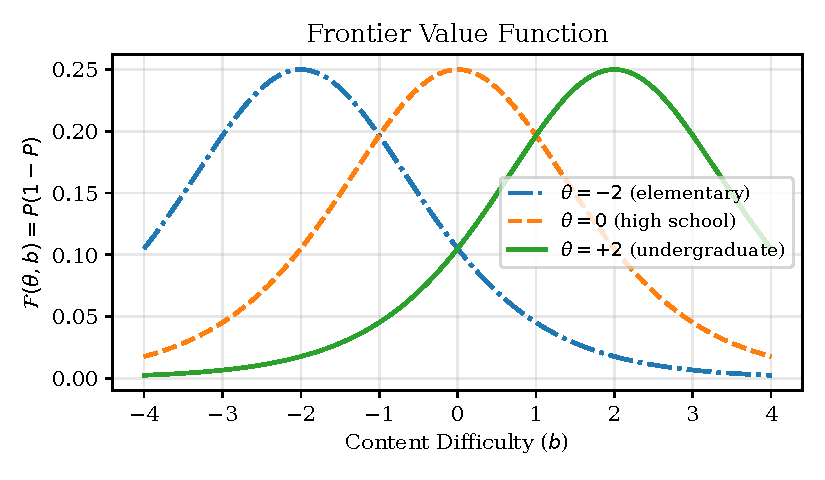
\includegraphics[width=0.75\linewidth]{fig1_frontier_value.pdf}
    \caption{Frontier Value $\mathcal{F}(\theta, b)$ for three ability levels. Selection concentrates around each user's frontier.}
    \label{fig:frontier}
\end{figure}

\subsection{PCR$^2$: Estimating $\theta$ from User Covariates}

The key extension. Let $\mathbf{Z}_j \in \mathbb{R}^p$ be observable covariates for user $j$ (education level, reading frequency, domain familiarity, age, vocabulary level). We decompose ability:
\begin{equation}
    \theta_j = \mathbf{Z}_j^{\mathrm{PC}} \boldsymbol{\gamma} + \varepsilon_j, \qquad \mathbf{Z}^{\mathrm{PC}} = \mathrm{PCA}(\mathbf{Z})
    \label{eq:pem}
\end{equation}
where $\mathbf{Z}^{\mathrm{PC}}$ is the PCA-compressed covariate matrix, $\boldsymbol{\gamma}$ are regression weights, and $\varepsilon_j$ is the residual person effect. This is the \emph{Person Explanatory Model} from the EIRM taxonomy~\cite{deboeck2004}.

\textbf{Cold-start prediction.} For a new user with no interaction history, $\varepsilon_j$ is unknown. We predict:
\begin{equation}
    \hat\theta_j^{\mathrm{cold}} = \mathbf{Z}_j^{\mathrm{PC}} \boldsymbol{\gamma}
\end{equation}

\textbf{Joint estimation.} All parameters ($\boldsymbol{\gamma}$, $\{\varepsilon_j\}$, $\{b_i\}$) are estimated jointly under the IRT likelihood:
\begin{equation}
    \mathcal{L} = \prod_{(j,i) \in \mathrm{obs}} P_{ji}^{x_{ji}} (1-P_{ji})^{1-x_{ji}}, \qquad P_{ji} = \sigma\!\left(\mathbf{Z}_j^{\mathrm{PC}} \boldsymbol{\gamma} + \varepsilon_j - b_i\right)
\end{equation}
avoiding the two-step bias that arises when estimated $\hat\theta$ values are used as regression outcomes~\cite{adams1997, deboeck2004}.

\textbf{Why PCA?} Raw user covariates are correlated (education correlates with vocabulary, age with reading frequency). PCA decorrelates and compresses, reducing the effective parameter count and avoiding multicollinearity.

\subsection{Difficulty Estimation}

PCR requires difficulty estimates $\hat{b}_i$. We evaluate:

\textbf{LLTM features}~\cite{fischer1973}: $\hat{b}_i = \sum_f w_f q_{if}$ with five handcrafted text features (sentence-length variance, long-word ratio, mean sentence length, inverse type-token ratio, average word length) and the fixed weights of Kang~\cite{kang2026pcr} ($w = [1.5, 0.8, 0.6, 1.2, 0.3]$). The feature set is modified relative to that work: feature~5 is average word length, whereas Kang~\cite{kang2026pcr} uses the frequency of context-dependency words; and mean sentence length is normalized by 30 rather than 20. The weights were carried over unchanged and were not re-fit for these modified features.

\textbf{Assigned labels}: Author- or curriculum-assigned difficulty levels, validated by LLM rating ($\rho=0.919$ in the original PCR paper).

\subsection{Full Pipeline}

\begin{algorithm}[t]
\caption{PCR$^2$ Routing}
\label{alg:pcr2}
\begin{algorithmic}[1]
\REQUIRE User covariates $\mathbf{Z}_j$, content chunks $\{c_i\}_{i=1}^N$, budget $K$, trained $\boldsymbol{\gamma}$
\STATE $\hat\theta_j \leftarrow \mathrm{PCA}(\mathbf{Z}_j) \cdot \boldsymbol{\gamma}$ \COMMENT{Cold-start: covariates only}
\FOR{each chunk $c_i$}
    \STATE Estimate $\hat{b}_i$ via LLTM features or cached labels
    \STATE $\mathcal{F}_i \leftarrow \hat{P}_i(1-\hat{P}_i)$, \quad $\hat{P}_i = \sigma(\hat\theta_j - \hat{b}_i)$
\ENDFOR
\STATE Select top-$K$ chunks by $\mathcal{F}_i$
\STATE Feed selected chunks to LLM for generation
\end{algorithmic}
\end{algorithm}

Computational cost of steps 1--5: one matrix multiply, $N$ sigmoid evaluations, one sort. Sub-millisecond for $N < 10{,}000$.

\section{Experimental Setup}

\subsection{Corpus}

58 Wikipedia article summaries across four difficulty levels: \textit{easy} (15 articles, e.g., ``Water'', ``Sun''), \textit{medium} (12, e.g., ``Photosynthesis'', ``DNA''), \textit{hard} (15, e.g., ``Enzyme'', ``Superconductivity''), \textit{expert} (16, e.g., ``Quantum entanglement'', ``Bose--Einstein condensate''). Summaries retrieved via the Wikipedia REST API
\url{/page/summary/} endpoint. LLTM features computed on actual summary text.

\subsection{Users}

100 synthetic user profiles with five observable covariates (education years, reading frequency, domain familiarity, age, vocabulary level) generated with controlled correlation to true $\theta \in [-2.6, +3.1]$: each covariate is a linear function of true $\theta$ plus Gaussian noise, clipped to a plausible range. No interaction-history covariates are used, ensuring an interaction-free cold-start simulation. Response matrix: $100 \times 58$ with 35\% sparsity; binary responses are drawn from the Rasch model using true $\theta$ and the assigned $b$. Only the passage text is real; users, covariates, responses, and the relevance model (Section~\ref{sec:strategies}) are synthetic.

\subsection{Strategies}
\label{sec:strategies}

\begin{enumerate}
    \item \textbf{Oracle PCR}: True $\theta$, assigned $b$ (upper bound).
    \item \textbf{PCR$^2$ cold-start}: $\hat\theta = \mathbf{Z}^{\mathrm{PC}}\boldsymbol{\gamma}$, assigned $b$.
    \item \textbf{PCR$^2$+LLTM}: $\hat\theta$ from covariates, $\hat{b}$ from LLTM features (fully API-free).
    \item \textbf{Simulated relevance oracle}: A Gaussian relevance model centered on true $\theta$, providing an upper bound on what perfect query-based retrieval could achieve if users always queried at their own level.
    \item \textbf{PCR+Relevance hybrid}: Relevance oracle retrieves top-$2K$, PCR reranks to top-$K$.
    \item \textbf{Difficulty-only}: Always selects the $K$ hardest passages.
    \item \textbf{Easiest-only}: Always selects the $K$ easiest passages.
    \item \textbf{Random}: Uniform random $K$ of $N$.
\end{enumerate}

Budget: $K=8$ of 58 passages (14\%).

\subsection{Metrics}

\textbf{Frontier value captured}: $\sum_{i \in \mathrm{sel}} \mathcal{F}(\theta_{\mathrm{true}}, b_i)$. Higher means better frontier match.

\section{Results}

\subsection{Ability Estimation Quality}

PCR-IRT latent regression achieves a Pearson correlation $r(\hat\theta, \theta_{\mathrm{true}}) = 0.963$ (Spearman $\rho = 0.961$) in cold-start mode (covariates only) and $R^2(\mathrm{person}) = 0.867$ (Figure~\ref{fig:theta}). Three principal components capture 92.4\% of covariate variance.

\begin{figure}[t]
    \centering
    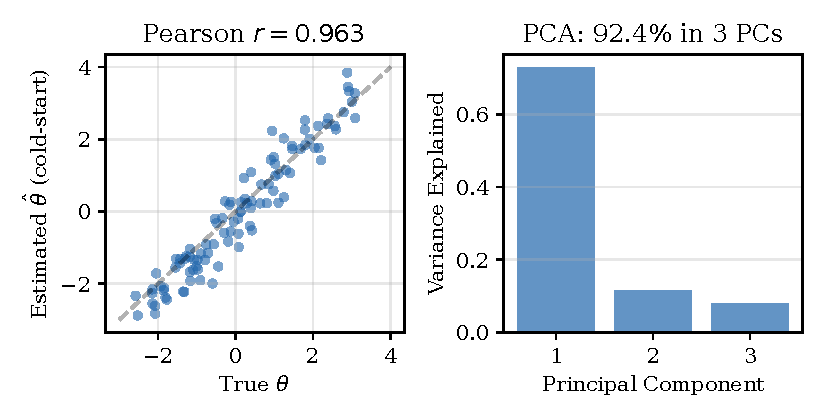
\includegraphics[width=\linewidth]{fig2_theta_estimation.pdf}
    \caption{Left: Cold-start $\hat\theta$ vs true $\theta$. Right: PCA variance explained.}
    \label{fig:theta}
\end{figure}

\subsection{LLTM Feature Failure}

LLTM handcrafted features achieve only $\rho=0.068$ ($p=0.61$) on Wikipedia text (Figure~\ref{fig:lltm}). The ``Water'' article has \emph{higher} sentence-length variance (0.396) than ``Quantum field theory'' (0.283) because encyclopedic prose normalizes surface complexity. Readability features cannot distinguish conceptual difficulty within the same register. This falsifies the ``API-free'' claim for heterogeneous corpora.

\begin{figure}[t]
    \centering
    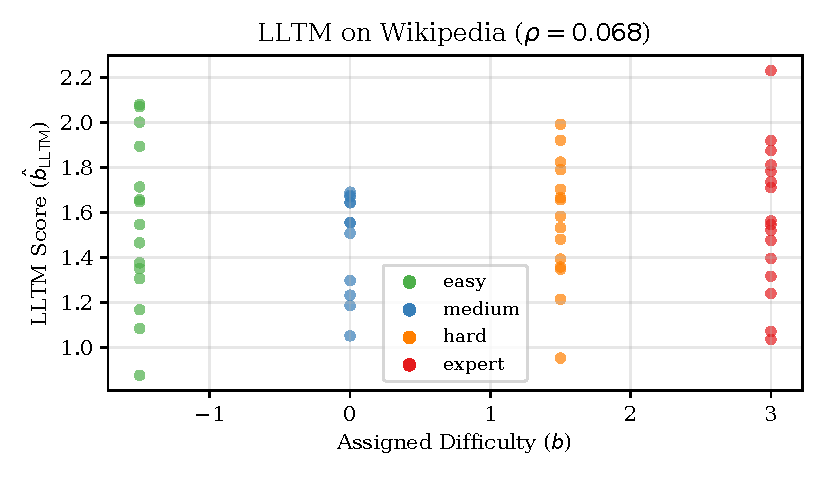
\includegraphics[width=0.75\linewidth]{fig3_lltm_failure.pdf}
    \caption{LLTM features vs.\ assigned difficulty on Wikipedia text ($\rho = 0.068$, essentially zero).}
    \label{fig:lltm}
\end{figure}

\subsection{Routing Quality}

\begin{table}[t]
\centering
\caption{Routing quality: frontier value captured (8 of 58 passages, 100 users). Bootstrap 95\% CIs from 10{,}000 resamples.}
\label{tab:main}
\begin{tabular}{lccccc}
\toprule
Strategy & Mean $\pm$ Std & \% Oracle & 95\% CI & $d$ vs Diff & $p$ \\
\midrule
Oracle PCR & $1.911 \pm 0.089$ & 100.0 & --- & --- & --- \\
Sim.\ relevance oracle & $1.900 \pm 0.098$ & 99.4 & [1.879, 1.918] & --- & --- \\
PCR+Rel.\ hybrid & $1.889 \pm 0.107$ & 98.8 & [1.866, 1.908] & 1.97 & $<10^{-15}$ \\
PCR$^2$ cold-start & $1.851 \pm 0.180$ & 96.9 & [1.811, 1.882] & 1.84 & $<10^{-15}$ \\
Easiest-only & $1.118 \pm 0.685$ & 58.5 & --- & 0.36 & 0.0005 \\
PCR$^2$+LLTM & $1.062 \pm 0.132$ & 55.6 & --- & 0.58 & $<0.001$ \\
Random & $1.003 \pm 0.292$ & 52.5 & [0.942, 1.057] & --- & --- \\
Difficulty-only & $0.645 \pm 0.635$ & 33.8 & [0.531, 0.782] & --- & --- \\
\bottomrule
\end{tabular}
\end{table}

Table~\ref{tab:main} presents the central results. PCR$^2$ cold-start captures 96.9\% of oracle quality. Against difficulty-only: $d=1.84$, 86/100 wins, $p<10^{-15}$.

\textbf{Critical finding}: The simulated relevance oracle achieves 99.4\% of oracle quality. This upper bound models a scenario where users always formulate queries at their own difficulty level, so that relevance-based retrieval implicitly selects difficulty-appropriate content. PCR$^2$ does not beat this oracle. However, in same-topic multi-level corpora where all documents are equally relevant but differ in difficulty, relevance alone cannot distinguish them and PCR$^2$ provides the missing signal.

Figure~\ref{fig:comparison} shows strategy comparison and per-ability selections.

\begin{figure}[t]
    \centering
    \begin{subfigure}[t]{0.48\linewidth}
        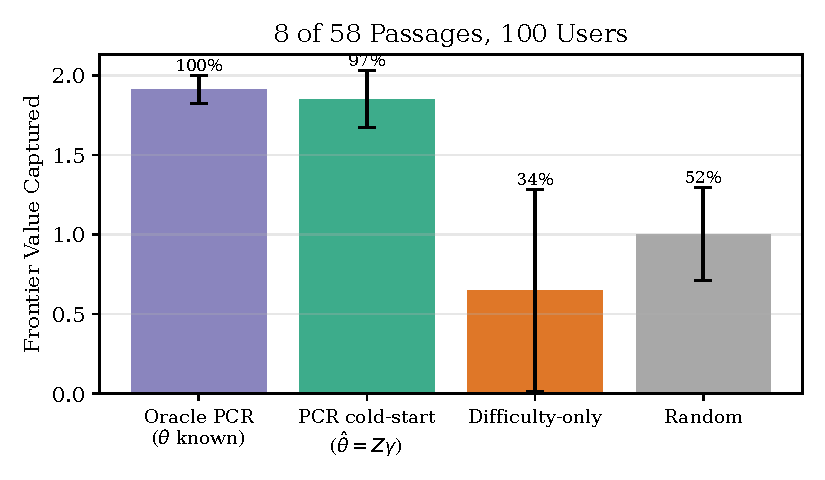
\includegraphics[width=\linewidth]{fig4_strategy_comparison.pdf}
        \caption{Strategy comparison}
    \end{subfigure}
    \hfill
    \begin{subfigure}[t]{0.48\linewidth}
        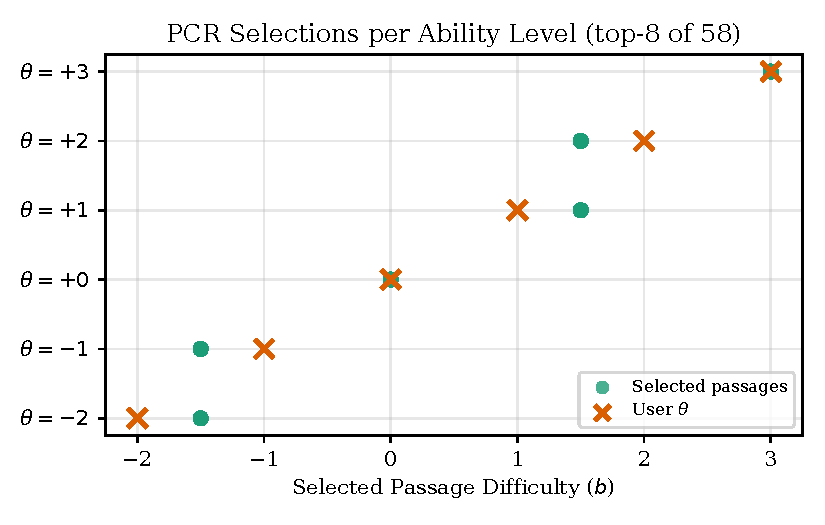
\includegraphics[width=\linewidth]{fig5_per_ability.pdf}
        \caption{Per-ability selections}
    \end{subfigure}
    \caption{(a)~Frontier value by strategy. (b)~PCR selects passages near each user's $\theta$.}
    \label{fig:comparison}
\end{figure}

\subsection{Scaling with Corpus Diversity}

Figure~\ref{fig:scaling_robust}(a) shows PCR advantage as a function of difficulty diversity $\sigma_b$. At low diversity ($\sigma_b = 0.43$), PCR provides $1.2\times$ advantage over random. At high diversity ($\sigma_b = 5.16$), the advantage reaches $3.5\times$ over random and $>400\times$ over difficulty-only (which collapses when extreme items dominate). The latter ratio is degenerate and should not be read as an effect size: at $\sigma_b = 5.16$, difficulty-only captures a mean frontier value of only 0.003 (vs.\ 1.40 for PCR and 0.40 for random), so the ratio is driven by a near-zero denominator. Note: the log scale is used because the difficulty-only ratio grows superlinearly.

\subsection{Robustness to Ability Estimation Noise}

Figure~\ref{fig:scaling_robust}(b) shows degradation under $\theta$ estimation noise. PCR maintains positive Cohen's $d$ against difficulty-only even at $\sigma_{\mathrm{noise}}=3.0$, and captures 65\% of oracle quality at that extreme. The method is robust because the frontier value function has a broad peak---neighboring passages still provide substantial $\mathcal{F}$.

\FloatBarrier
\begin{figure}[t]
    \centering
    \begin{subfigure}[t]{0.48\linewidth}
        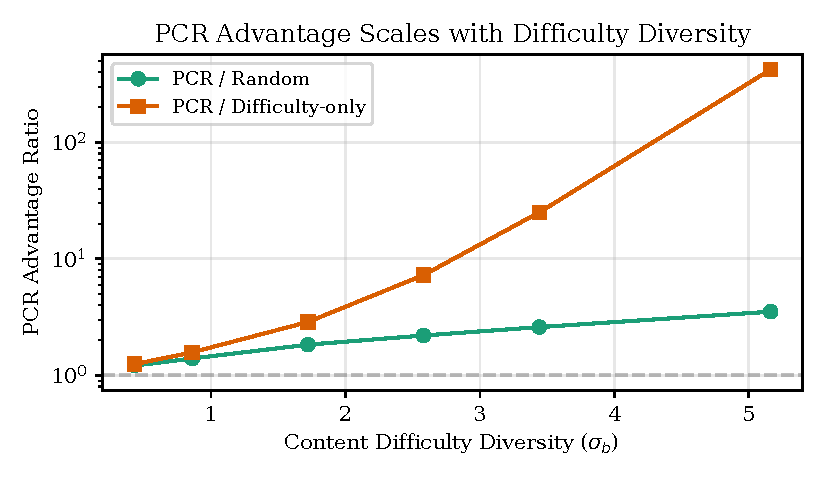
\includegraphics[width=\linewidth]{fig6_scaling.pdf}
        \caption{Scaling with diversity (log scale)}
    \end{subfigure}
    \hfill
    \begin{subfigure}[t]{0.48\linewidth}
        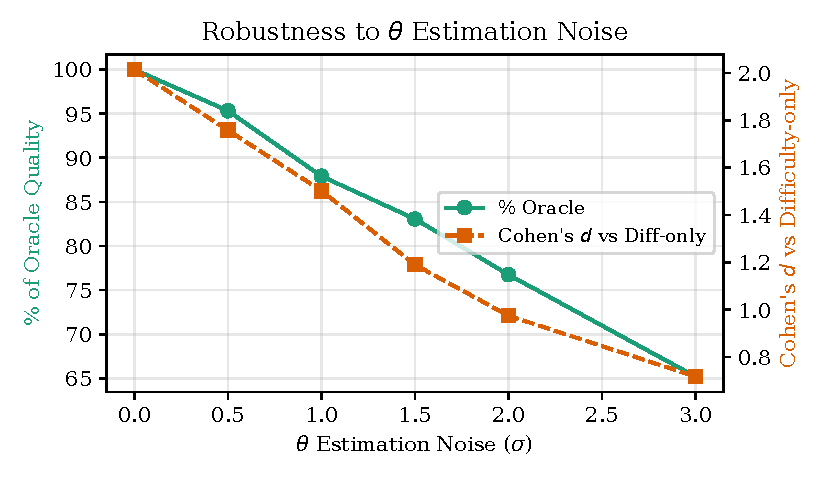
\includegraphics[width=\linewidth]{fig7_robustness.pdf}
        \caption{Noise robustness}
    \end{subfigure}
    \caption{(a)~PCR advantage grows with difficulty diversity. (b)~Robustness to $\theta$ estimation noise.}
    \label{fig:scaling_robust}
\end{figure}

\section{Discussion}

\subsection{When PCR Wins}

PCR$^2$ has a decisive advantage in \textbf{same-topic multi-level corpora}: knowledge bases where the same concept exists at multiple difficulty levels (beginner textbook through research monograph). Here, all documents are equally \emph{relevant} but differ in difficulty. Relevance-based retrieval cannot distinguish them; PCR$^2$ selects the difficulty-appropriate version. Real deployment scenarios include educational platforms with multi-level curricula, medical knowledge bases (patient-facing vs.\ clinician-facing content), technical documentation with beginner/advanced paths, and multi-level language learning corpora.

\subsection{When PCR Does Not Help}

In general-purpose RAG over heterogeneous corpora where users formulate queries at their own level, relevance-based retrieval implicitly achieves difficulty matching. PCR adds no value here. We consider this an important negative result.

\subsection{The LLTM Failure}

The five handcrafted readability features cannot distinguish conceptual difficulty within the same textual register. Wikipedia's ``Water'' article has comparable surface complexity to ``Quantum field theory.'' This is a \emph{category error}: readability $\neq$ conceptual difficulty. Future work should replace handcrafted features with learned difficulty embeddings (e.g., fine-tuned sentence-BERT), LLM-based difficulty rating ($\rho=0.919$ per Kang~\cite{kang2026pcr}), or curriculum-metadata-based difficulty.

\subsection{Relationship to EIRM Taxonomy}

PCR$^2$ instantiates the \emph{Person Explanatory Model} cell of the De Boeck \& Wilson~\cite{deboeck2004} EIRM taxonomy: $\theta_j = \mathbf{Z}_j\boldsymbol{\gamma} + \varepsilon_j$. Combined with LLTM on the item side ($b_i = \mathbf{Q}_i\mathbf{w} + \delta_i$), it becomes a \emph{Doubly Explanatory Model}. However, given the LLTM failure on real text, the item-explanatory component requires stronger features.

\FloatBarrier
\section{Limitations}

\begin{enumerate}
    \item \textbf{Simulated users.} User covariates and responses are synthetic with controlled covariate--ability correlation. Real user data would test whether this correlation holds in practice.
    \item \textbf{No human evaluation.} Frontier value is a proxy. Actual comprehension or learning outcome measurement is needed.
    \item \textbf{Small corpus.} 58 article summaries. Production systems have $10^4$--$10^6$ documents.
    \item \textbf{LLTM failure.} Handcrafted features do not work on encyclopedic text. The ``API-free'' pipeline is currently broken for heterogeneous corpora.
    \item \textbf{Simulated relevance oracle.} The relevance baseline is a thought experiment, not actual BM25 retrieval. Real retrieval experiments are needed.
    \item \textbf{Single difficulty dimension.} Real content varies along multiple axes (conceptual, linguistic, domain-specific).
\end{enumerate}

\section{Conclusion}

PCR$^2$ demonstrates an interaction-free $\theta$-estimation pathway for Psychometric Content Routing via PCA-compressed latent regression. In synthetic simulation, the method captures 96.9\% of oracle routing quality with $d=1.84$ against difficulty-only selection. However, the real-text smoke test (real Wikipedia text; synthetic users, covariates, responses, and relevance) reveals that (1)~LLTM handcrafted features fail on real text, requiring learned difficulty estimation, and (2)~a simulated relevance oracle achieves near-perfect routing, limiting PCR's advantage to same-topic multi-level corpora where relevance alone cannot distinguish difficulty. We provide complete code, data, and negative results to support reproducible evaluation.

\section*{Reproducibility}

The supplementary archive contains: \LaTeX\ source and all seven figures; 58 Wikipedia article summaries with LLTM features; user profile generation; experiment runner with bootstrap CIs; figure generation. Code and data: \url{https://github.com/testofschool/pcr-squared}

\bibliographystyle{plainnat}
\bibliography{references}

\end{document}
